\documentclass[11pt, a4paper]{article}

% --- Packages ---
\usepackage[utf8]{inputenc}
\usepackage[T1]{fontenc}
\usepackage{geometry}
\geometry{top=2.5cm, bottom=2.5cm, left=2.5cm, right=2.5cm}
\usepackage{mathptmx} % Times-like font
\usepackage{amsmath, amssymb, amsfonts}
\usepackage{graphicx}
\usepackage{booktabs} % For professional tables
\usepackage{hyperref}
\usepackage{authblk}  % For author affiliations
\usepackage{lineno}   % Line numbers for review
\usepackage{color}
\usepackage[sort&compress,numbers]{natbib}
\usepackage{caption}
\usepackage{float}    % For figure placement

% --- Hyperlink Settings ---
\hypersetup{
    colorlinks=true,
    linkcolor=blue,
    filecolor=magenta,      
    urlcolor=cyan,
    citecolor=blue,
}

% --- Title & Authors ---
\title{\textbf{PocketGNN: Enzyme Kinetic Parameter Prediction via Graph Neural Networks and Active Pocket Structural Characterization}}

\author[1]{Zihao Li}
\author[1,*]{Diannan Lu}

\affil[1]{Department of Chemical Engineering, Tsinghua University, Beijing, China}
\affil[*]{Corresponding author: ludiannan@tsinghua.edu.cn}

\date{}

\begin{document}

\maketitle

% \linenumbers 

% =======================================================
% ABSTRACT
% =======================================================
\begin{abstract}
\noindent
\textbf{Motivation:} Enzyme kinetic parameters, particularly the Michaelis constant ($K_{M}$) and catalytic constant ($k_{cat}$), are critical for assessing enzyme-substrate affinity and catalytic efficiency. With the advent of protein sequence generation models, there is an urgent need for efficient and accurate prediction of these parameters to facilitate high-throughput screening. Traditional experimental methods are often costly and inefficient for large-scale applications, while existing sequence-based computational methods struggle to capture the fine-grained structural nuances of the active site.

\noindent
\textbf{Results:} We propose PocketGNN, a structure-aware graph neural network framework for the efficient prediction of $K_{M}$ and $k_{cat}$. The framework integrates an automated pipeline comprising protein structure acquisition (ESMFold/PDB), substrate 3D modeling, and molecular docking (AutoDock Vina) to explicitly extract the active pocket. The core module, PocketGNNWithAttention, employs a Graph Attention Network (GAT) to learn atomic-level features, innovatively incorporating Gaussian Radial Basis Function (RBF)-encoded edge features and experimental temperature as a global contextual embedding. Validated on a diverse dataset derived from IntEnzyDB, PocketGNN achieved determination coefficients ($R^{2}$) of 0.884 for $\log_{10}(K_{M})$ and 0.918 for $\log_{10}(k_{cat})$, significantly outperforming sequence-based baselines. Furthermore, interpretability analysis using Input $\times$ Gradient successfully identified key catalytic residues, aligning well with biochemical knowledge.

\noindent
\textbf{Availability:} Source code and data are available at https://github.com/RektonLee/PGNN.

\noindent
\textbf{Keywords:} Enzyme kinetics; Graph Neural Networks; Active pocket; Molecular docking; Deep learning
\end{abstract}

% =======================================================
% 1. INTRODUCTION
% =======================================================
\section{Introduction}
\label{sec:intro}

Enzymes are indispensable biological catalysts that orchestrate metabolic networks and drive biotransformations. Two fundamental kinetic parameters, the Michaelis constant ($K_M$) and the turnover number ($k_{cat}$), quantitatively describe enzymatic performance: the former measures substrate affinity, while the latter reflects catalytic efficiency at saturation \cite{srinivasan2023guide}. Accurate determination of these parameters is vital for understanding catalytic mechanisms, guiding rational enzyme design, and accelerating drug discovery. However, traditional experimental assays are labor-intensive, time-consuming, and expensive, making them ill-suited for the rapid screening requirements of modern synthetic biology and enzyme engineering.

Recent advances in deep learning offer a promising alternative. Early data-driven approaches primarily relied on protein sequences, utilizing descriptors or pre-trained language models (e.g., ESM-1b) to predict kinetic properties \cite{kroll2021deep, yu2023unikp}. While scalable, these sequence-based methods often lack explicit 3D structural information, failing to capture the local spatial arrangements of the active site that directly govern catalysis. This limitation becomes critical when distinguishing enzymes with high sequence similarity but distinct kinetic behaviors due to subtle structural variations.

With the breakthrough of AlphaFold2 and ESMFold, acquiring high-quality protein structures has become feasible at scale. This has paved the way for structure-aware modeling. However, existing structural models often process the entire protein structure, introducing noise from non-catalytic regions, or fail to adequately model the specific physicochemical environment of the enzyme-substrate interaction interface.

To address these challenges, we introduce PocketGNN, a framework centered on the 3D structure of the enzyme active pocket. Unlike previous methods, PocketGNN employs an automated molecular docking pipeline to capture the realistic binding pose of the substrate. We construct a local graph representation of the active pocket and utilize a Graph Attention Network (GAT) enhanced with Gaussian Radial Basis Function (RBF) edge features to model fine-grained atomic interactions. Additionally, we integrate experimental temperature as a global feature to account for environmental effects. Our model demonstrates superior predictive accuracy and provides structural interpretability, offering a powerful tool for next-generation enzyme design.

% =======================================================
% 2. MATERIALS AND METHODS
% =======================================================
\section{Materials and Methods}
\label{sec:methods}

\subsection{Dataset Construction and Preprocessing}
Data was curated from IntEnzyDB \cite{yan2022intenzydb}, encompassing 686 enzymes, 2540 single-point mutants, and 929 distinct substrates. We filtered the dataset to retain entries with valid UniProt IDs, substrate SMILES strings, and experimental kinetic values measured at known temperatures. To ensure model stability, extreme outliers were removed, resulting in a final high-quality dataset of 3,025 unique enzyme-substrate pairs covering all six main EC classes.
The target variables, $K_M$ and $k_{cat}$, span multiple orders of magnitude and were therefore log-transformed ($\log_{10}$) to facilitate regression stability.

\subsection{Automated Active Pocket Extraction}
A key innovation of our framework is the automated extraction of the active pocket based on docked conformations (Figure \ref{fig:framework}).
\begin{itemize}
    \item \textbf{Structure Acquisition:} Enzyme structures were retrieved from the PDB or predicted using ESMFold when experimental structures were unavailable. Substrate 3D conformers were generated from SMILES using RDKit with UFF energy minimization.
    \item \textbf{Molecular Docking:} We employed AutoDock Vina for docking. Potential binding sites were identified using AutoSite to define the search box. The pose with the lowest binding affinity was selected as the representative complex structure.
    \item \textbf{Pocket Definition:} The active pocket was defined as the subset of protein atoms within a 5.0 \AA{} radius of any substrate atom in the docked complex. This significantly reduces input dimensionality while retaining the most relevant catalytic information.
\end{itemize}

\begin{figure}[htbp]
    \centering
    \includegraphics[width=\textwidth]{Architecture.png}
    % \fbox{\begin{minipage}{\textwidth}
    %     \centering
    %     \vspace{2cm}
    %     \textbf{[Figure 1: Overall Framework of PocketGNN]} \\
    %     \small This figure should illustrate the pipeline: Dataset -> Structure Acquisition (ESMFold) -> Docking (AutoDock Vina) -> Pocket Extraction -> Graph Construction -> GNN Model -> Prediction.
    %     \vspace{2cm}
    % \end{minipage}}
    \caption{The overall framework of PocketGNN. The pipeline integrates automated structure generation, molecular docking for pocket extraction, and a graph neural network for kinetic parameter prediction.}
    \label{fig:framework}
\end{figure}

\subsection{Graph Representation}
The extracted active pocket is modeled as a graph $G=(V, E)$.
\textbf{Nodes ($V$):} Each atom is a node characterized by a feature vector encoding element type, residue type, ligand indicator (binary), nearest neighbor distance, electronic state, and physicochemical properties (mass, electronegativity).
\textbf{Edges ($E$):} Edges are constructed between atoms within a spatial cutoff of 4.0 \AA. To capture precise geometric relationships, edge features are encoded using Gaussian Radial Basis Functions (RBF) to represent continuous distances in a high-dimensional space.

\subsection{Model Architecture}
The core model, PocketGNNWithAttention, consists of the following components:
\begin{enumerate}
    \item \textbf{Node Encoder:} Projects initial atomic features into a hidden space.
    \item \textbf{Graph Attention Layers (GAT):} We stack 6 GAT layers to update node representations. A multi-head attention mechanism (8 heads) allows the model to dynamically weigh the importance of neighboring atoms. Crucially, RBF-encoded edge features are integrated into the attention mechanism to inject spatial constraints.
    \item \textbf{Global Pooling \& Temperature Fusion:} Node features are aggregated via global mean pooling. The experimental temperature is normalized and embedded via a separate MLP, then fused with the graph representation. This allows the model to adjust predictions based on reaction conditions.
    \item \textbf{Regression Head:} A final MLP predicts $\log_{10}(K_M)$ and $\log_{10}(k_{cat})$.
\end{enumerate}

% =======================================================
% 3. RESULTS AND DISCUSSION
% =======================================================
\section{Results and Discussion}
\label{sec:results}

\subsection{Performance Evaluation}
We compared PocketGNN against several baselines, including sequence-based models (Sequence Baseline, Sequence Enhanced with ChemBERTa) and structure-based methods without attention mechanisms (PGNN-Basic). The models were trained on 80\% of the data and validated on 20\%.

As shown in Table \ref{tab:performance}, PocketGNN (Full) achieved the best performance across all metrics. For $\log_{10}(k_{cat})$, it attained an $R^2$ of 0.918 and a Pearson correlation ($r$) of 0.98. For $\log_{10}(K_M)$, the $R^2$ was 0.884, with $r=0.98$. This significantly outperforms the Sequence Baseline ($R^2 < 0$), demonstrating the necessity of structural information.

% --- DEMO: LaTeX Table Insertion ---
\begin{table}[htbp]
  \centering
  \caption{Quantitative prediction results on the validation set.}
  \label{tab:performance}
  \begin{tabular}{lccccc}
    \toprule
    Model & MSE ($k_{cat}$) & $R^2$ ($k_{cat}$) & MSE ($K_M$) & $R^2$ ($K_M$) & Pearson $r$ \\
    \midrule
    Sequence Baseline & 2.227 & -30.15 & 14.99 & -2.76 & 0.18 \\
    Sequence Enhanced & 0.28 & -0.32 & 0.15 & 0.77 & 0.82 \\
    PGNN-Basic & 0.79 & 0.665 & 0.63 & 0.589 & 0.95 \\
    \textbf{PGNN-Full (Ours)} & \textbf{0.19} & \textbf{0.918} & \textbf{0.21} & \textbf{0.884} & \textbf{0.98} \\
    \bottomrule
  \end{tabular}
\end{table}
% --- END DEMO: LaTeX Table Insertion ---

Figure \ref{fig:scatter} visualizes the correlation between predicted and ground truth values. The density plots show a tight clustering around the diagonal $y=x$, indicating high prediction accuracy and low bias. Our model minimizes the overall loss function $\mathcal{L}$ for both parameters simultaneously, defined as:

% --- DEMO: LaTeX Equation Insertion ---
$$\mathcal{L} = \frac{1}{N}\sum_{i=1}^{N}\left((\log_{10}K_{M,i} - \overline{\log_{10}K_{M,i}})^2 + (\log_{10}k_{cat,i} - \overline{\log_{10}k_{cat,i}})^2\right)$$
% --- END DEMO: LaTeX Equation Insertion ---

\noindent where $\overline{x}$ denotes the model's predicted value. The high performance demonstrates effective joint modeling of the two kinetic parameters. The prediction scatter plots are shown in Figure \ref{fig:scatter}.

\begin{figure}[htbp]
    \centering
    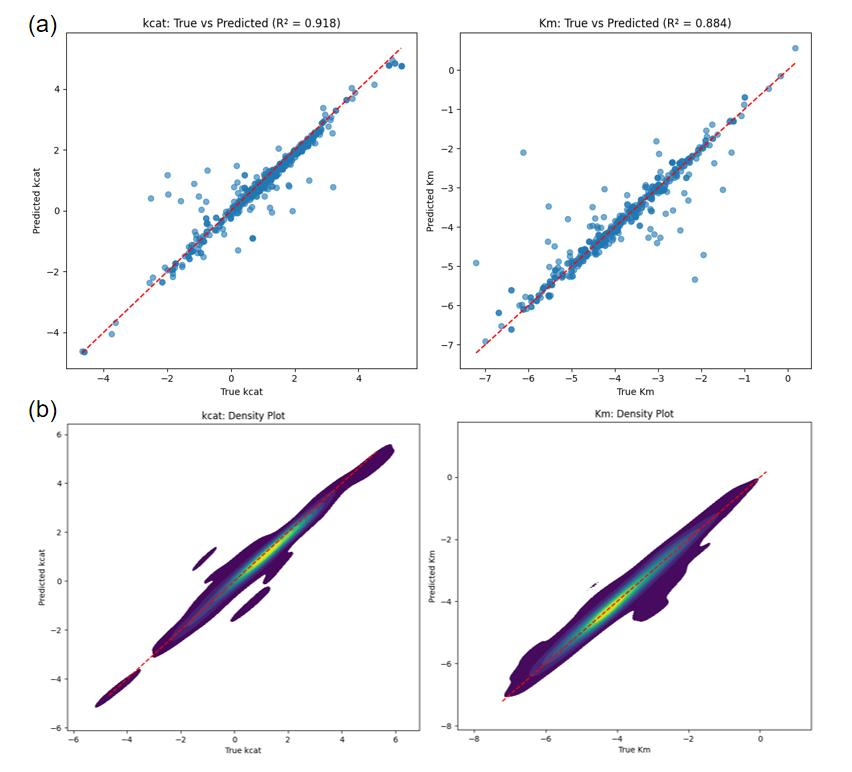
\includegraphics[width=0.8\textwidth]{scatter.png}
    % \fbox{\begin{minipage}{0.8\textwidth}
    %     \centering
    %     \vspace{1.5cm}
    %     \textbf{[Figure 3: Scatter and Density Plots]} \\
    %     \small Scatter plots of Predicted vs True values for both $k_{cat}$ and $K_M$, showing high correlation ($R^2 > 0.88$).
    %     \vspace{1.5cm}
    % \end{minipage}}
    \caption{Scatter plots and density heatmaps of true versus predicted values for (a) $\log_{10}(k_{cat})$ and (b) $\log_{10}(K_M)$ on the validation set.}
    \label{fig:scatter}
\end{figure}

\subsection{Ablation Studies}
We conducted ablation studies to verify the contribution of specific modules:
\begin{itemize}
    \item \textbf{Effect of RBF Edge Features:} Removing RBF encoding (using scalar distance only) caused an $R^2$ drop of approximately 7\% for $k_{cat}$, highlighting the importance of high-dimensional spatial encoding.
    \item \textbf{Effect of Temperature:} Excluding the temperature feature (PGNN$\backslash$T) resulted in a significant performance decline, confirming that experimental conditions are vital context for kinetic predictions.
    \item \textbf{Input Representation:} Comparing the docking-based pocket input vs. separate protein/ligand inputs (Prot\_GNN) showed that the explicit modeling of the complex interface is crucial for capturing interaction patterns.
\end{itemize}

\subsection{Interpretability and Case Study}
To validate the model's biological relevance, we employed the Input $\times$ Gradient method to visualize atomic contributions. Using Aldehyde Dehydrogenase (UniProt: P30838) as a case study, we mapped the saliency scores onto the 3D structure (Figure \ref{fig:case_study}).
The visualization reveals that atoms with high contribution scores (highlighted in red) are concentrated around the substrate binding pocket and catalytic residues (e.g., PRO205, ARG424). This suggests that PocketGNN successfully learns to focus on functionally relevant regions rather than relying on spurious correlations.

\begin{figure}[htbp]
    \centering
    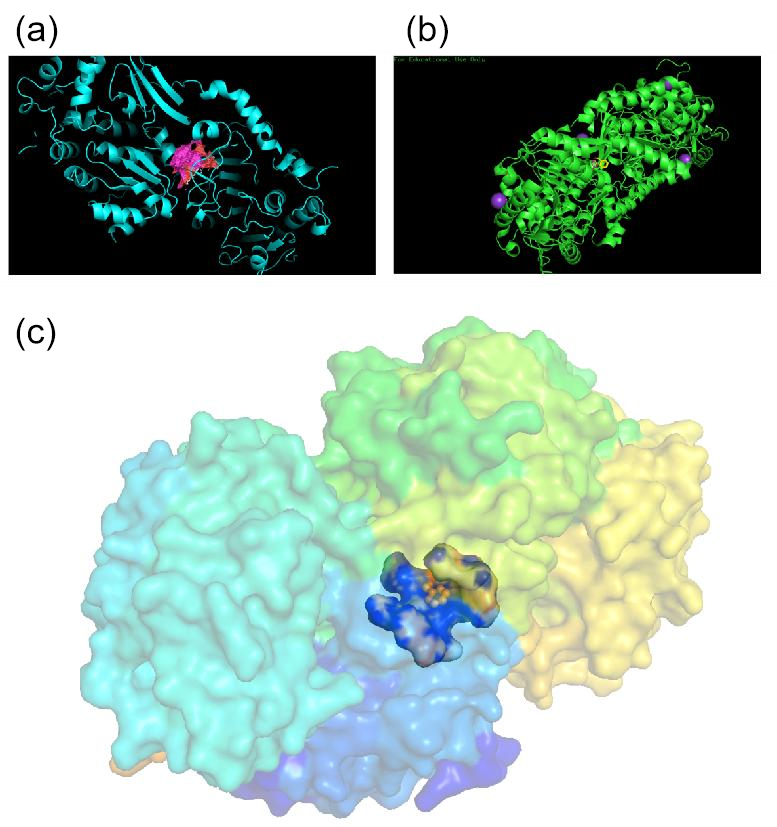
\includegraphics[width=0.7\textwidth]{visualize.png}
    % \fbox{\begin{minipage}{0.7\textwidth}
    %     \centering
    %     \vspace{2cm}
    %     \textbf{[Figure 4: Interpretability Visualization]} \\
    %     \small 3D visualization of the docked complex (P30838). Atoms are colored by saliency score (Input x Gradient), highlighting the active site.
    %     \vspace{2cm}
    % \end{minipage}}
    \caption{Visualization of atomic contributions for Aldehyde Dehydrogenase. High-saliency atoms (red) cluster around the catalytic center and substrate, validating the model's focus on the active pocket.}
    \label{fig:case_study}
\end{figure}

% =======================================================
% 4. CONCLUSION
% =======================================================
\section{Conclusion}
\label{sec:conclusion}

This study presents PocketGNN, an automated, interpretable, and high-precision deep learning framework for predicting enzyme kinetic parameters. By leveraging the 3D structure of the active pocket obtained via molecular docking and incorporating graph attention mechanisms with RBF edge encoding, our model significantly outperforms sequence-based approaches. The integration of experimental temperature further enhances robustness. Crucially, the model demonstrates the ability to identify key catalytic atoms, bridging the gap between "black-box" prediction and structural biology insights. PocketGNN provides a valuable computational tool for enzyme engineering and synthetic biology applications.

% =======================================================
% REFERENCES
% =======================================================
\bibliographystyle{unsrt}
\begin{thebibliography}{10}

\bibitem{srinivasan2023guide}
Srinivasan B. A guide to enzyme kinetics in early drug discovery. \textit{FEBS Journal}, 2023, 290(9): 2292-2305.

\bibitem{kroll2021deep}
Kroll A, Engqvist MKM, Heckmann D, et al. Deep learning allows genome-scale prediction of Michaelis constants from structural features. \textit{PLoS Biology}, 2021, 19(10): e3001402.

\bibitem{yu2023unikp}
Yu H, Deng H, He J, et al. UniKP: a unified framework for the prediction of enzyme kinetic parameters. \textit{Nature Communications}, 2023, 14(1): 8211.

\bibitem{yan2022intenzydb}
Yan B, Ran X, Gollu A, et al. IntEnzyDB: an Integrated Structure-Kinetics Enzymology Database. \textit{Journal of Chemical Information and Modeling}, 2022, 62(22): 5841-5848.

\bibitem{trott2010autodock}
Trott O, Olson AJ. AutoDock Vina: improving the speed and accuracy of docking with a new scoring function. \textit{Journal of Computational Chemistry}, 2010, 31(2): 455-461.

\bibitem{velickovic2018graph}
Velickovic P, Cucurull G, Casanova A, et al. Graph Attention Networks. \textit{ICLR}, 2018.

\end{thebibliography}

\end{document}